\section{Properties of the Community Cores}

In this section, we present a series of analyses about the scientific community cores. First, we analyze how the network properties of the scientific communities have evolved. %Section~\ref{sub:time}.
Then, we contrast the properties of the community cores over time against the properties of the remaining members of the respective communities. 
Finally, we compute the average core score of a community to investigate variations in the properties of the members of the core of each community and 
correlate these variations with the network properties of the communities.


\subsection{Evolution of the Scientific Communities}
\label{sub:time}

As an attempt to understand the main structural properties of the scientific communities, we examine the evolution of the structure of their networks on the light of complex
network analysis. To do so, we calculated various network metrics for each of the scientific communities. We present four popular metrics here: assortativity, average clustering
coefficient, average path length, and the size of the largest weakly connected component (WCC). Figure~\ref{fig:metrics} shows how each of these four metrics vary over time
for a set of six scientific communities selected among those that spam over the longest period in our dataset.  Our analysis are performed under two perspectives. The first
consists on analyzing the network evolution year by year of accumulating nodes and edges to a single final snapshot of the graph. This perspective allow us to observe the final
network structure of a community as a function of time. The second perspective consists of analyzing snapshots constructed based on nodes and edges created on an predefined time
window (three years, as discussed in Section~\ref{sub:thresholds}). This analysis allows us to investigate network variations with potential to impact the final network structure.
Our analysis results are similar for the other communities, but we omit them due to lack of space.

We note from Figure~\ref{fig:metrics} that the largest WCC tend to largely increase as a function of time. This suggests that at early
stages, scientific communities are formed by several small and segregated research groups. With time, some reserachers (e.g., students) leave an institute and begin collaborations
with other research groups. Additionally, as the community evolves, heads of  research groups tend to colabrate with other peers of the same community. Thus, with time, authors
from different groups tend to collaborate and increase the size of the largest WCC. As a consequence, the average shortest path, computed only on the largest
WCC, tends to increase, becoming stable around typical small-world values (i.e., from 4 to 10 hops)~\cite{mislove-2007-socialnetworks,fourdegrees_facebook}.  We can
also note that the average clustering coefficient tends to values between 0.1 and 0.2, thus suggesting that the coauthors of an author have 10\% to 20\% of chance to be connected
among themselves. These values tend to slightly diminishe over time, as small components tend to connect to form larger components reducing the average clustering coefficient
value.  When it comes to assortativity, we see that this measure tends to 0, but it is still positive. This means that there is a slight tendency in these communities of nodes to
connect with others with similar degree.  A positive value for assortativity is a typical characteristic of sociological networks~\cite{Newman2003}.

In general, we can note that scientific communities have similar evolving characteristics and these properties are dynamic as they change over time.  More important, our
observations suggest that a small set of authors are responsible for the social clue that creates the paths among smaller and more connected research groups. Next, we seek to
further investigate this group of authors. To that end, in the next subsection we propose an approach to identify the authors' core of scientific communities.



\begin{figure}[!htb]
  \begin{center}
  \subfigure[Final Assortativity]{%
    \label{fig:assortativity_1_in_1}
    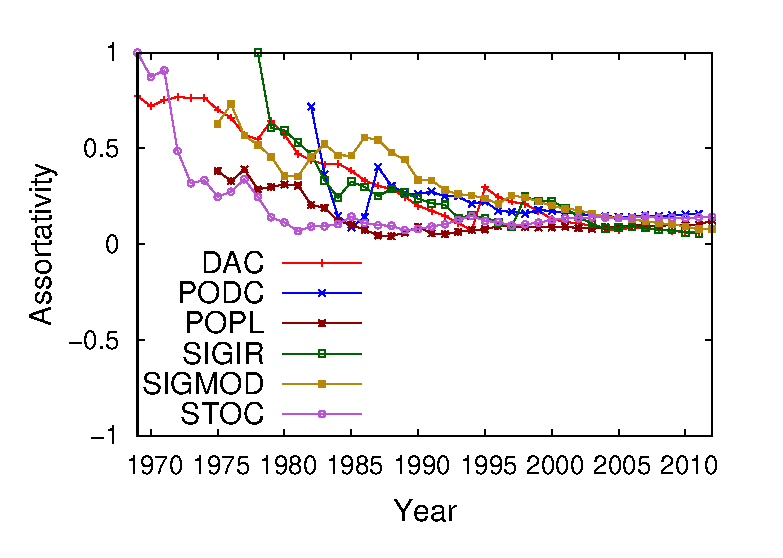
\includegraphics[scale=.33]{graficos/sigs_metricas_acumuladas_1_em_1_ano/assortatividade_grupo_temporal_web.eps}
  }%
  \subfigure[Assortativity per Window]{%
    \label{fig:assortativity_slide_window}
    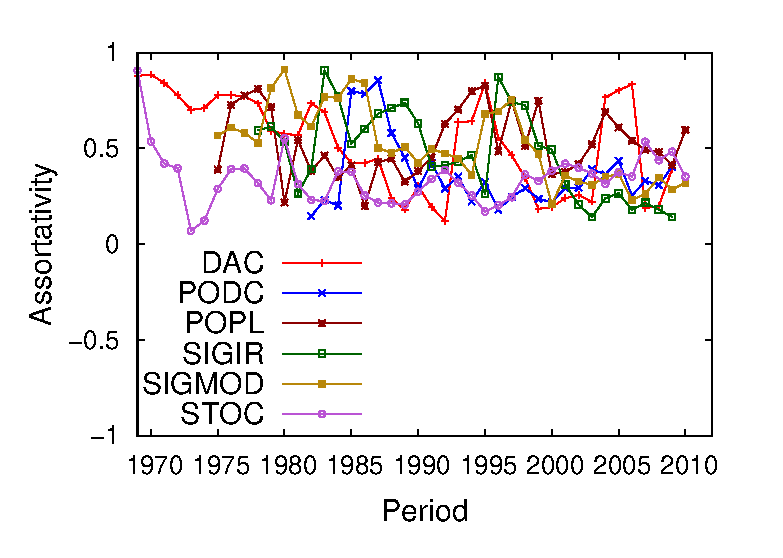
\includegraphics[scale=.33]{graficos/core_over_time/metricas_tradicionais/assortatividade_slide_window_grupo_temporal_web.eps}
  }%
  \\
  \subfigure[Final average shortest path]{%
    \label{fig:average_shortest_path_1_in_1}
    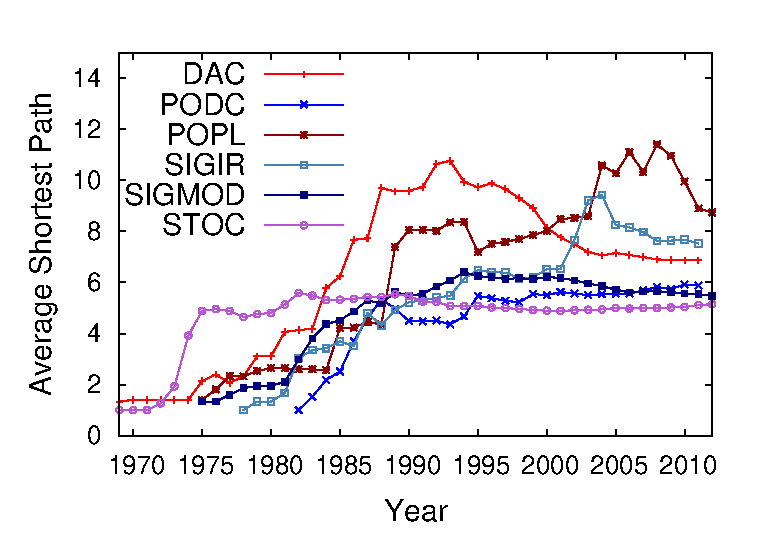
\includegraphics[scale=.33]{graficos/sigs_metricas_acumuladas_1_em_1_ano/caminho_minimo_medio_grupo_temporal_web.eps}
  }%
  \subfigure[Avg. shortest path per window]{%
    \label{fig:average_shortest_path_slide_window}
    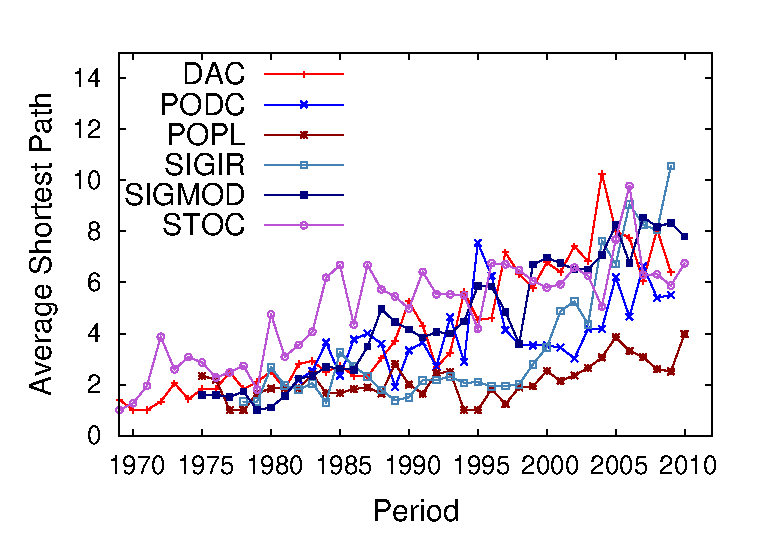
\includegraphics[scale=.33]{graficos/core_over_time/metricas_tradicionais/caminho_minimo_medio_slide_window_grupo_temporal_web.eps}
  }%
  \\
  \subfigure[Final clustering coefficient]{%
    \label{fig:clustering_coefficient_1_in_1}
    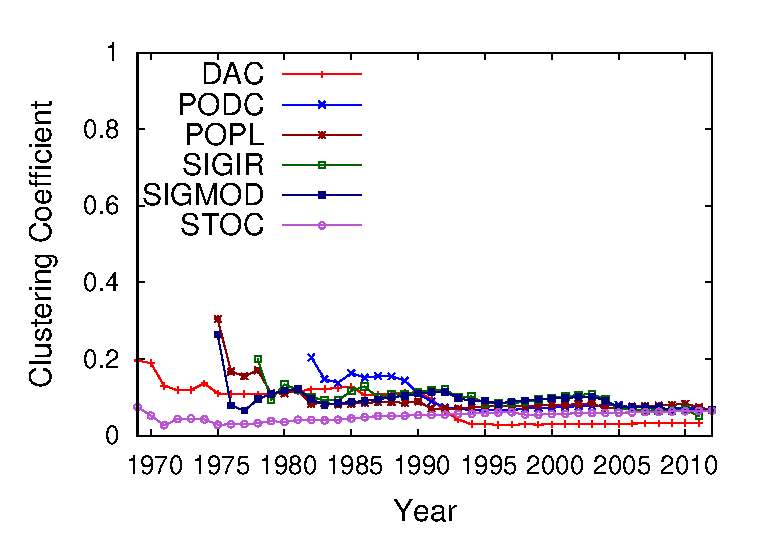
\includegraphics[scale=.33]{graficos/sigs_metricas_acumuladas_1_em_1_ano/coeficiente_agrupamento_grupo_temporal_web.eps}
  }%
  \subfigure[Clustering coefficient per window]{%
    \label{fig:clustering_coefficient_slide_window}
    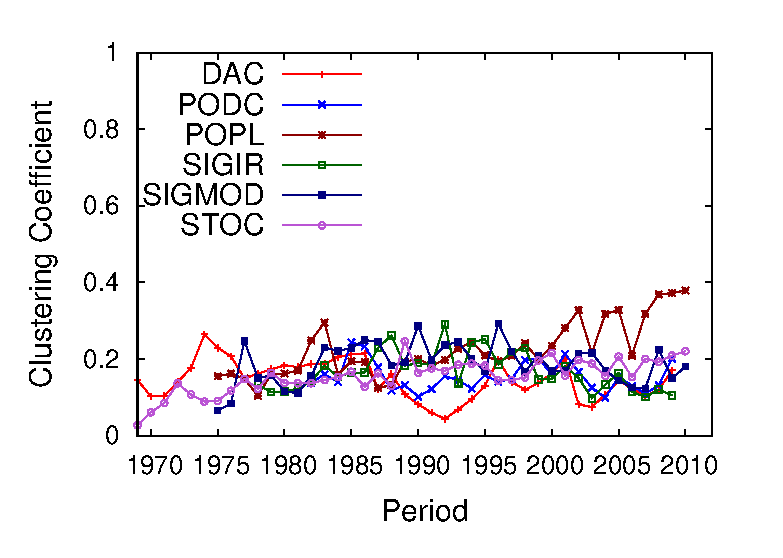
\includegraphics[scale=.33]{graficos/core_over_time/metricas_tradicionais/coeficiente_agrupamento_slide_window_grupo_temporal_web.eps}
  }%
  \\
  \subfigure[Final largest WCC]{%
    \label{fig:largest_connected_component_1_in_1}
    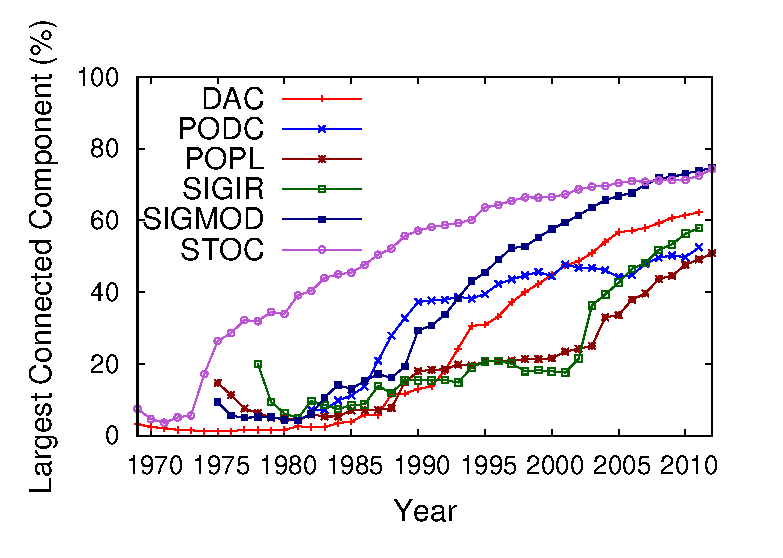
\includegraphics[scale=.33]{graficos/sigs_metricas_acumuladas_1_em_1_ano/porcentagem_maior_componente_grupo_temporal_web.eps}
  }%
  \subfigure[Largest WCC per window]{%
    \label{fig:largest_connected_component_slide_window}
    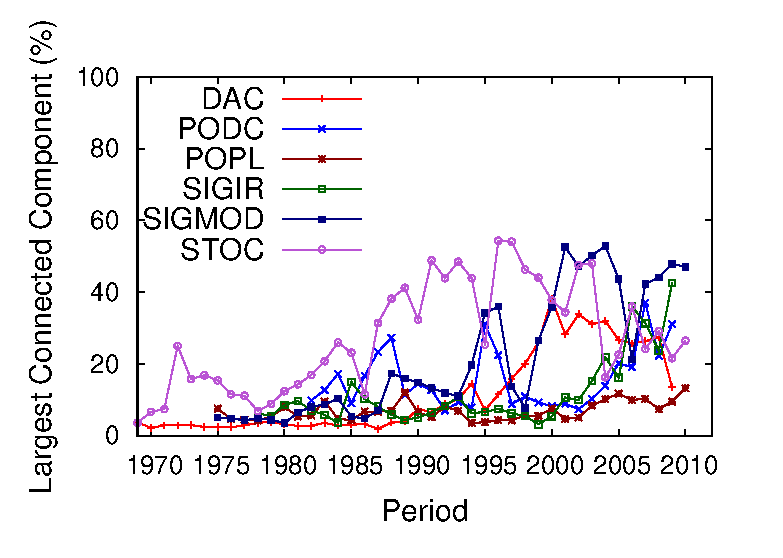
\includegraphics[scale=.33]{graficos/core_over_time/metricas_tradicionais/porcentagem_maior_componente_slide_window_grupo_temporal_web.eps}
  }%
  \\
  \subfigure[Final average degree]{%
    \label{fig:average_degree_1_in_1}
    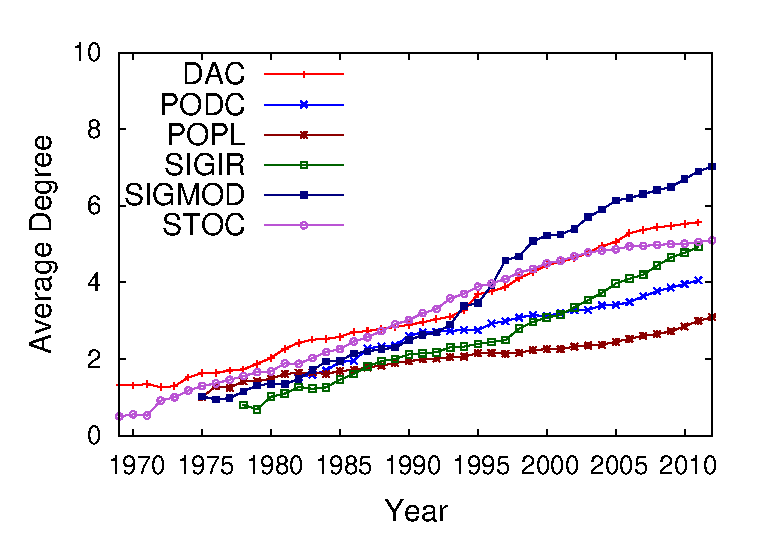
\includegraphics[scale=.33]{graficos/sigs_metricas_acumuladas_1_em_1_ano/grau_medio_nodos_grupo_temporal_web.eps}
  }%
  \subfigure[Avg. degree per window]{%
    \label{fig:average_degree_slide_window}
    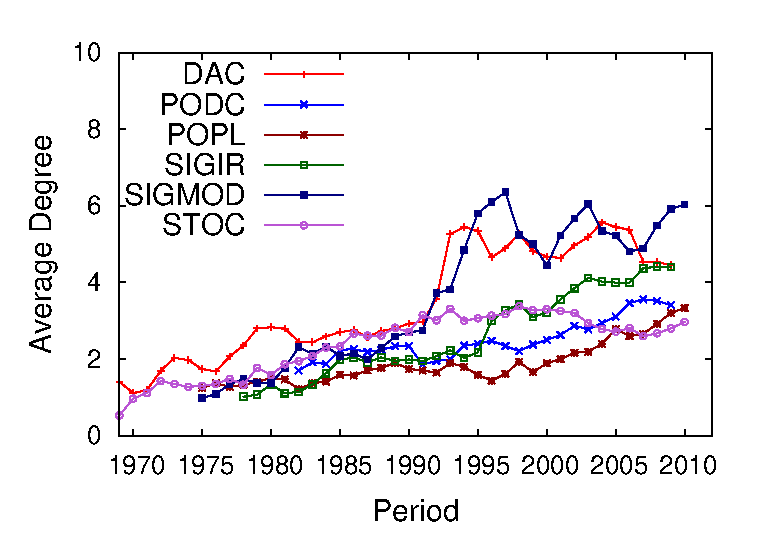
\includegraphics[scale=.33]{graficos/core_over_time/metricas_tradicionais/grau_medio_nodos_slide_window_grupo_temporal_web.eps}
  }%
  \end{center}
  \caption{Network evolution metrics for scientific communities}
  \label{fig:metrics}
\end{figure}



\subsection{Core vs. Other Members}
\label{sub:vs}

To what extend the properties of the core community differ from the rest of the community?  Next, we compute node network properties for members and non-members of the core
community. We consider the time window analysis to understand the variations that these two classes might have in the global measure.
Figure~\ref{fig:metrics_comparing_core_community} shows the average degree and the average clustering coefficient computed by the members and non-members of the SIGMOD core
community. Additionally, we also measure the fraction of community core members as well as non-members that are in the largest WCC. We can make key observations
from theses analysis. First, we can note that the average degree of the members of the core considerably higher in comparison with non-members, as they tend to establish more and
more connections as a function of time. However, the clustering coefficient of the members of the core tend to be slightly smaller in comparison with non-members meaning that they
might act like hubs, by connecting different groups with small intersection. Indeed, by analyzing the fraction of members of the core community that are part of the largest
WCC, we can note that it is much larger than the fraction of non-members, suggesting that they might be connecting smaller components. Next, we investigate how
aspects of the members of a core community can impact in the overall structure of the community.


\begin{figure*}[!htb]
  \begin{center}
  \subfigure[Clustering coefficient]{%
    \label{fig:core_com_sigmod_clustering_coefficient}
    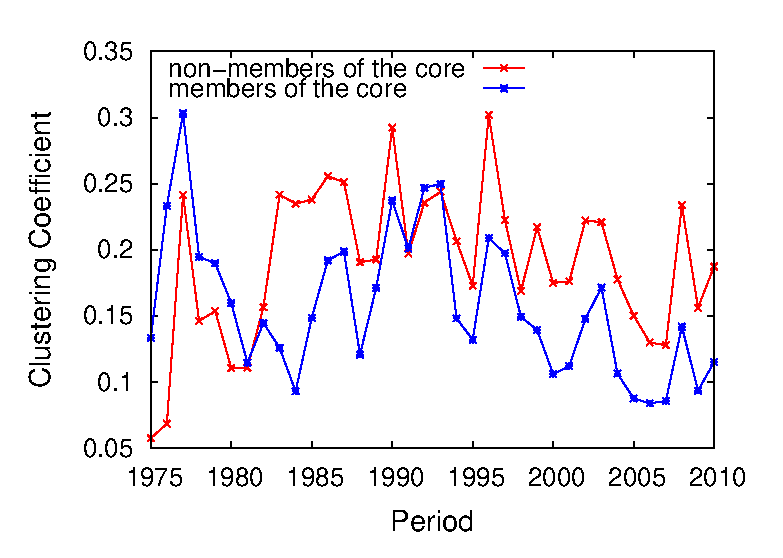
\includegraphics[scale=.33]{graficos/core_over_time/core_community/sigmod_janela_3_core_coeficiente_agrupamento.eps}
  }%
  \subfigure[Avg. Degree]{%
    \label{fig:core_com_sigmod_average_degree}
    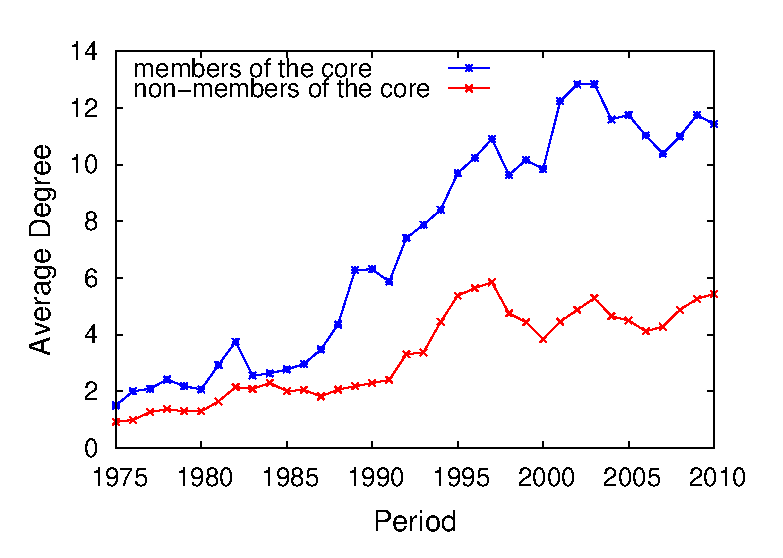
\includegraphics[scale=.33]{graficos/core_over_time/core_community/sigmod_janela_3_core_grau_medio_nodos.eps}
  }%
  \subfigure[Largest WCC]{%
    \label{fig:core_com_sigmod_largest_connected_component}
    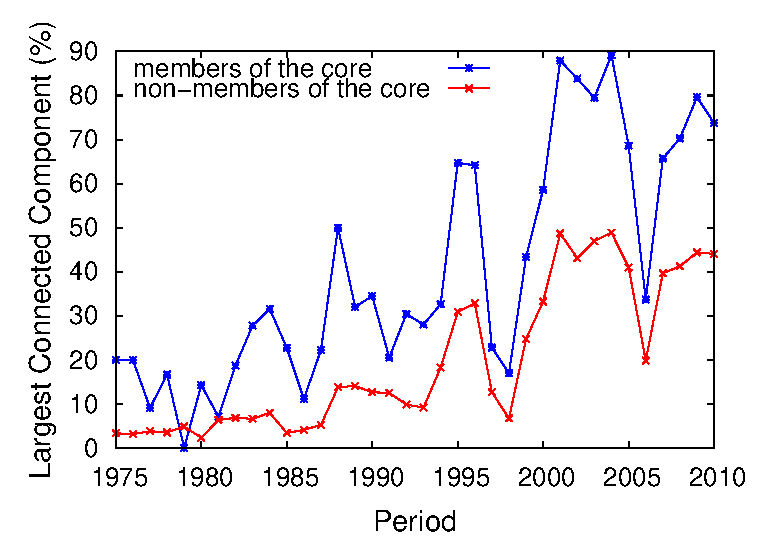
\includegraphics[scale=.33]{graficos/core_over_time/core_community/sigmod_janela_3_core_maior_componente_conectado.eps}
  }%
  \subfigure[Avg. Betweenness]{%
    \label{fig:core_com_sigmod_betweenness}
    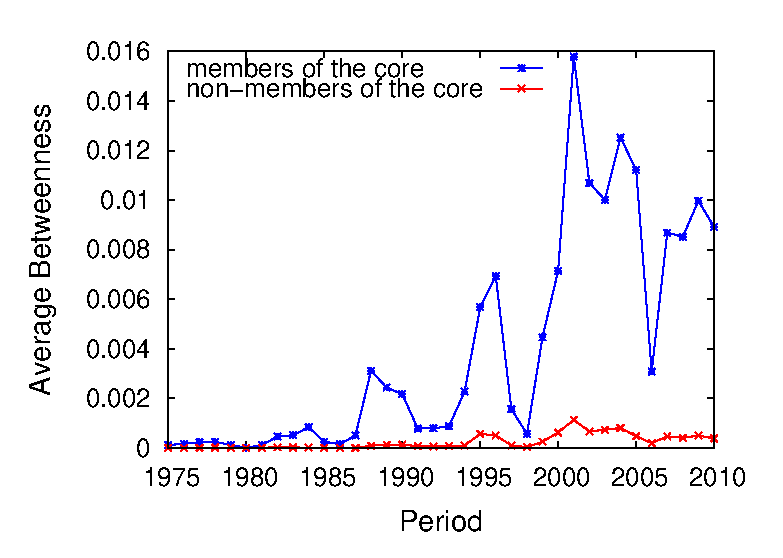
\includegraphics[scale=.33]{graficos/core_over_time/core_community/sigmod_janela_3_core_betweenness.eps}
  }%
  \end{center}
  \caption{SIGMOD network properties for members and non-members of the core}
  \label{fig:metrics_comparing_core_community}
\end{figure*}



\subsection{Core Communities and Network Structure}
\label{sub:corr}

We now examine to what extent the community core fluctuations affect the network structure.  To that end, we compute the average core score of the members of each community over
time. Intuitively, this measure captures the overall proliftness and involvement of the core members of a scientific community. Figure~\ref{fig:average_core_score} shows this value
for a set of communities as a function of time. We plot it in two separate figures to facilitate visualization. We can note that all communities experimented rises and falls along
its life time, indicating strong variations in the core score values of the members of the core. We can speculate innumerous factors that are able to explain such variations,
including expansion or reduction in the number of published papers, raise and fall of hot topics with ability to attract or loose important core members, members involved in the
conference organization, etc. However, disregarding what caused the variations, we want to investigate if such variations can directly impact the network structure.


\begin{figure}[!htb]
  \begin{center}
    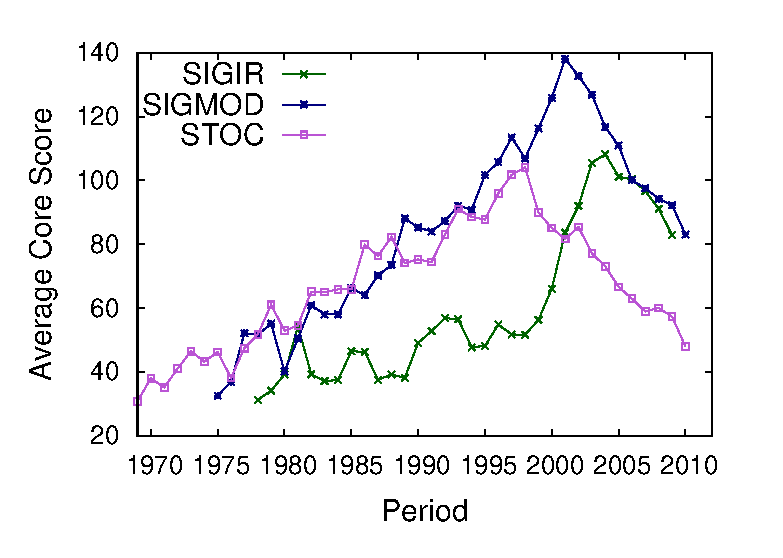
\includegraphics[scale=.325]{graficos/average_core_score/average_core_score_slide_window_grupo_1_temporal_web.eps}
    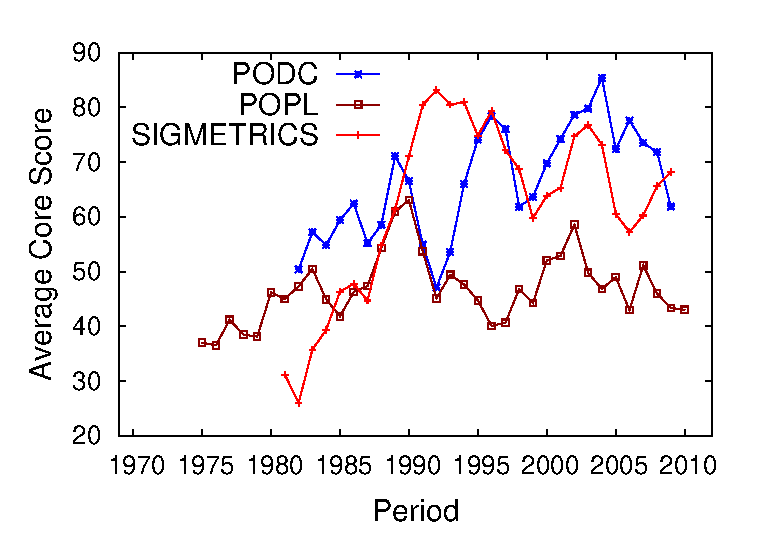
\includegraphics[scale=.325]{graficos/average_core_score/average_core_score_slide_window_grupo_2_temporal_web.eps}
  \end{center}
  \caption{Avg. core score of scientific communities}
  \label{fig:average_core_score}
\end{figure}


Our approach to investigate this issue, consists of computing the pearson correlation coefficient between the average core score of each scientific community and a number of
network metrics for that community.  Table~\ref{tab:correlation_metrics} presents these values.

We make key observations from these analysis. First, we can note that the Diameter of a conference is positive correlated with the average core score. Although for some communities
we cannot see values close to 0 or even negative values (e.g. Mobicom, with -0.04), the average correlation coefficient for all communities is 0.49, which indicates an overall
positive tendency. This means that when the average core score of a community increases or decreases, the diameter tends to follow the same tendency. This suggests that core score
members might connect smaller components, creating bridges among them, which contributes to increase the overall diameter. This conjecture is also supported by the high coefficient
correlation for the average shortest path (in average 0.49) and the size of the largest WCC (in average 0.5).

Second, we can note that a highly positive correlation coefficient between the average core score of communities and the average degree of the network.  However, we can also
observe a strong negative correlation with the assortativeness of the network. This suggests that an increase in the average community core increases the set of highly connected
nodes in the network. Although they create paths among components, they tend to connect themselves mostly with nodes of small degree values, decreasing the assortativeness of the
network. Indeed, a senior researcher might tend to be co-author of a high number of students and young researchers, but also keep collaborations with other senior researchers from
other groups.

Finally, despite some variations, we note a clear pattern for most of the conferences on each of the analyzed metrics (i.e. clear positive or negative correlations for most of the
communities). This reinforces that our observations holds for a significant number of scientific communities. 


%We measured each of these metrics for samples of the graph obtained at each time window as we did in previous analysis.

\begin{table*}[!htb]
\centering
\caption{Corelation between average core score of the communities core and network metrics}
\label{tab:correlation_metrics}
{\small
\begin{tabular}{|l|c|c|c|c|c|c|} \hline
& \bf Diameter & \bf Avg. Short P. & \bf Clus. Coef. & \bf Assort. & \bf Larg. WCC & \bf Avg. Deg. \\ \hline
CCS & 0.34 & 0.2 & 0.23 & -0.2 & 0.45 & 0.14 \\ \hline
CHI & 0.75 & 0.79 & -0.62 & -0.74 & 0.76 & 0.77 \\ \hline
CIKM & 0.56 & 0.56 & -0.52 & -0.67 & 0.39 & 0.87 \\ \hline
DAC & 0.8 & 0.85 & -0.49 & -0.63 & 0.76 & 0.92 \\ \hline
HSCC & 0.17 & 0.45 & -0.62 & -0.71 & 0.87 & 0.55 \\ \hline
ICSE & 0.81 & 0.83 & -0.52 & -0.84 & 0.68 & 0.8 \\ \hline
ISCA & 0.63 & 0.55 & 0.54 & -0.32 & 0.63 & 0.81  \\ \hline
ISSAC & 0.05 & 0.01 & -0.25 & -0.43 & -0.07 & 0.21 \\ \hline
KDD & 0.1 & 0.17 & -0.33 & -0.67 & 0.2 & 0.14\\ \hline
MICRO & 0.35 & 0.35 & 0.28 & -0.36 & 0.52 & 0.51 \\ \hline
MOBICOM & -0.04 & 0.11 & 0.13 & -0.65 & 0.23 & -0.09 \\ \hline
Multimedia & 0.67 & 0.68 & -0.91 & -0.95 & 0.67 & 0.69 \\ \hline
PODC & 0.4 & 0.42 & -0.23 & -0.2 & 0.13 & 0.68 \\ \hline
POPL & 0.21 & 0.2 & 0.23 & -0.43 & 0.25 & 0.19 \\ \hline
SAC & 0.48 & 0.59 & 0.16 & -0.39 & -0.55 & 0.16 \\ \hline
SIGCOMM & 0.18 & 0.19 & 0.05 & -0.81 & 0.49 & 0.41\\ \hline
SIGCSE & 0.88 & 0.84 & -0.22 & -0.5 & 0.93 & 0.87 \\ \hline
SIGDOC & 0.73 & 0.78 & -0.36 & -0.89 & 0.66 & 0.76 \\ \hline
SIGGRAPH & 0.79 & 0.85 & -0.45 & -0.75 & 0.94 & 0.88 \\ \hline
SIGIR & 0.83 & 0.85 & -0.42 & -0.77 & 0.7 & 0.89 \\ \hline
SIGMETRICS & 0.31 & 0.24 & 0.3 & -0.44 & 0.37 & 0.64 \\ \hline
SIGMOD & 0.78 & 0.81 & 0.27 & -0.61 & 0.77 & 0.87 \\ \hline
SIGUCCS & 0.38 & -0.22 & 0.53 & -0.13 & 0.51 & 0.7 \\ \hline
STOC & 0.61 & 0.63 & 0.54 & -0.37 & 0.82 & 0.88\\ \hline \hline
{\bf Average} & {\bf 0.49} & {\bf 0.49} & {\bf -0.11} & {\bf -0.56} & {\bf 0.5} & {\bf 0.59} \\ \hline
\end{tabular}
}
\end{table*}



